\documentclass[10pt]{article}
\usepackage{longtable}
\usepackage{float}
\usepackage{wrapfig}
\usepackage{rotating}
\usepackage[normalem]{ulem}
\usepackage{amsmath}
\usepackage{textcomp}
\usepackage{marvosym}
\usepackage{wasysym}
\usepackage{amssymb}
\usepackage{hyperref}
\usepackage{graphicx}
\graphicspath{{/Users/benjaminbass/seacloud/class/earthMaterials/mineralSheets/tectosilicates/leucite/images/}}

\usepackage{frame,color}
\usepackage{framed}
\usepackage{minibox}

% \usepackage[T1]{fontenc}
% \usepackage{tilting} %bring title up
% \setlength{\droptitle}{-10cm} 

\usepackage[version=3]{mhchem}

%How to Use MChem
% \ce{SO4^2-}
% \ce{^{227}_{90}Th+}
% \ce{A\bond{-}B\bond{=}C\bond{#}D}
% \ce{CO2 + C -> 2CO}
% \ce{SO4^2- + Ba^2+ -> BaSO4 v}

\author{Benjamin Bass}
\date{24 February2016}
\title{\vspace{-2.0cm}Leucite} %bring title up temporary Fix

\begin{document}

\maketitle

\begin{center}
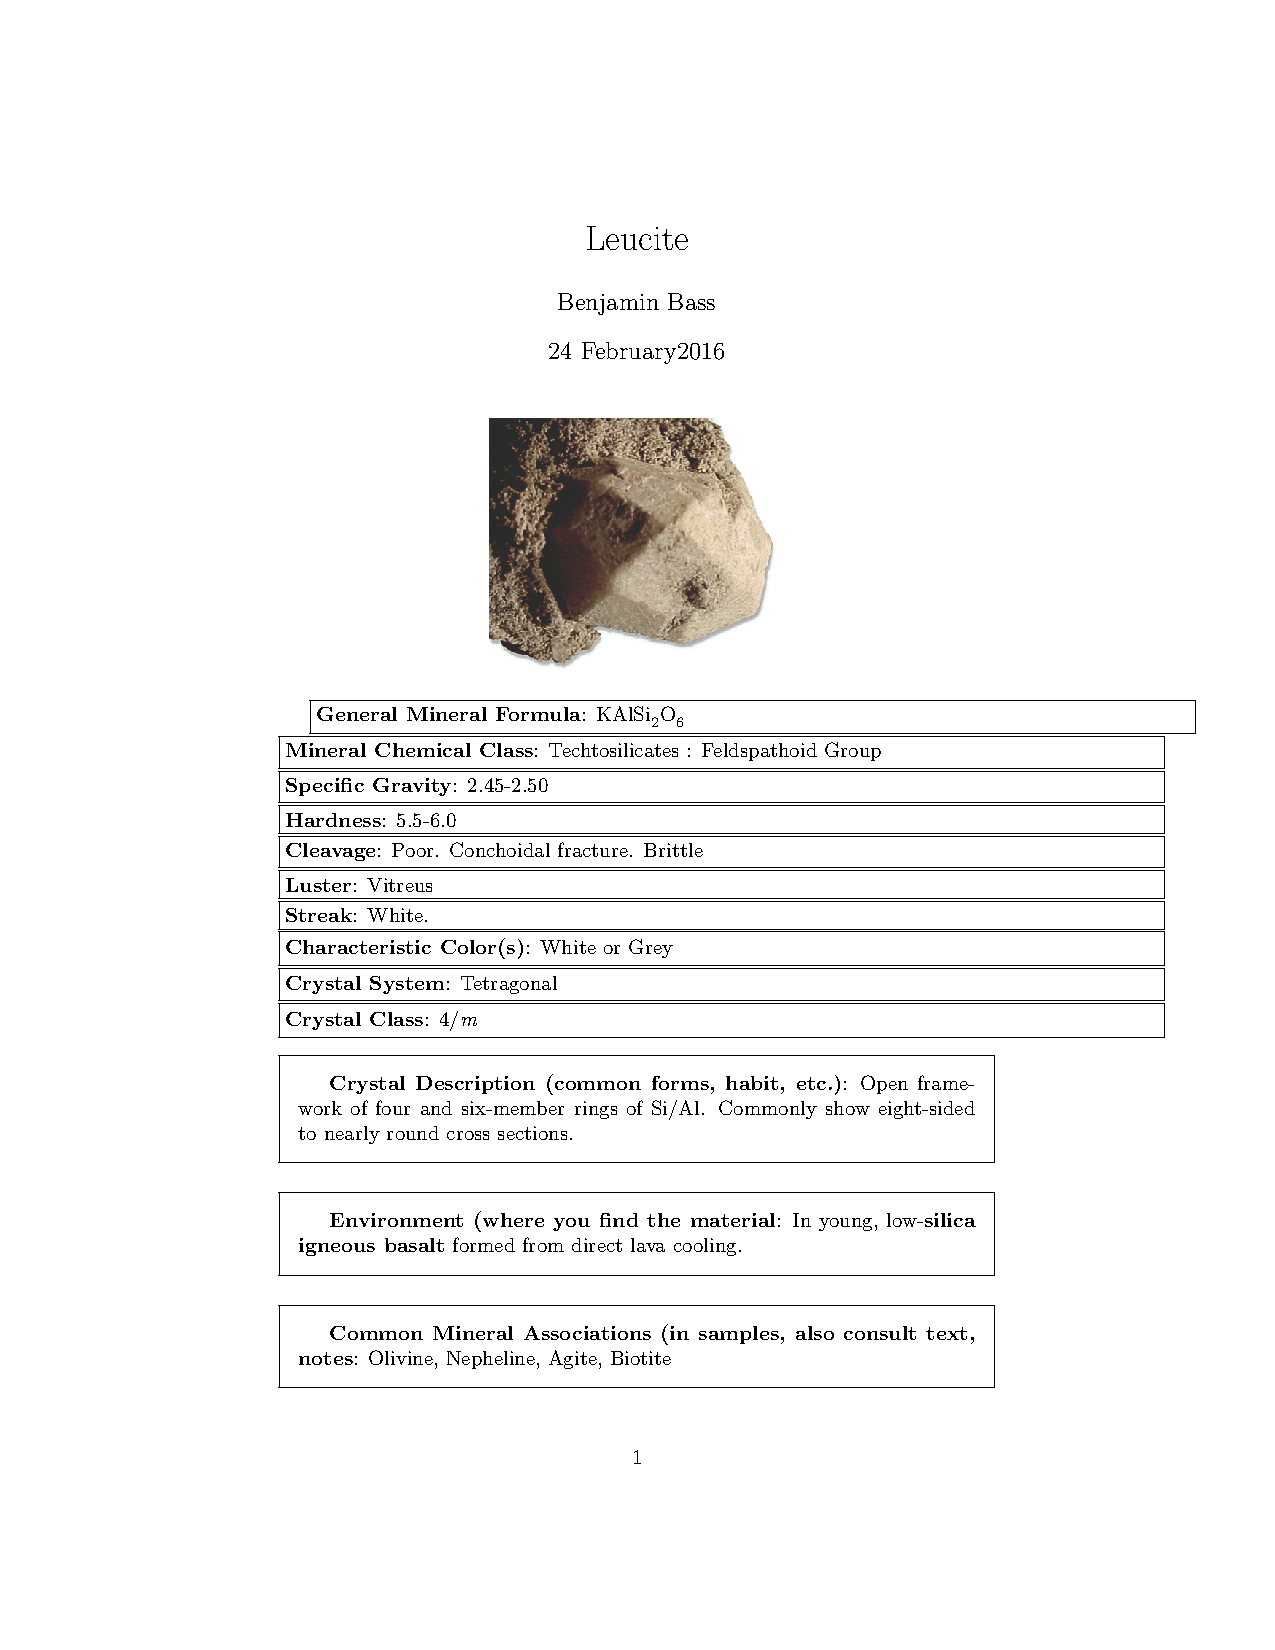
\includegraphics[scale=.35]{leucite}
\end{center}

% \framebox{Use frameboxes until figure out alignmen}

\framebox[15cm][l]{\textbf{General Mineral Formula}: \ce{KAlSi_2O_6} }\    
\framebox[15cm][l]{\textbf{Mineral Chemical Class}: Techtosilicates : Feldspathoid Group }\
\framebox[15cm][l]{\textbf{Specific Gravity}: 2.45-2.50 }\
\framebox[15cm][l]{\textbf{Hardness}: 5.5-6.0 }\
\framebox[15cm][l]{\textbf{Cleavage}:  Poor. Conchoidal fracture. Brittle }\
\framebox[15cm][l]{\textbf{Luster}:  Vitreus }\
\framebox[15cm][l]{\textbf{Streak}: White.}\
\framebox[15cm][l]{\textbf{Characteristic Color(s)}:  White or Grey }\
\framebox[15cm][l]{\textbf{Crystal System}: Tetragonal}\
\framebox[15cm][l]{\textbf{Crystal Class}: 4/\it{m}}\

\begin{framed}
  \textbf{Crystal Description (common forms, habit, etc.)}: Open framework of four and six-member rings of Si/Al. Commonly show eight-sided to nearly round cross sections.
\end{framed}

\begin{framed}
  \textbf{Environment (where you find the material}:  In young, low-\textbf{silica igneous basalt} formed from direct lava cooling.
\end{framed}

\begin{framed}
  \textbf{Common Mineral Associations (in samples, also consult text, notes}:  Olivine, Nepheline, Agite, Biotite
\end{framed}

\begin{framed}
  \textbf{Scientific Usage/Significance}: None
\end{framed}

\begin{framed}
  \textbf{Industrial or Social Use/Significance}:  Used in the manufacture of ceramics and in dental prostheses.
\end{framed}

\begin{framed}
  \textbf{Environmental Significance}:  Fertilizer for its potassium content.
\end{framed}

% Possible other Solutions
% \framebox(300,20){\minibox{\textbf{R-Sq}:For example}}

\end{document}
%%% Local Variables:
%%% mode: latex
%%% TeX-master: t
%%% End: